\chapter{Native Elongating Transcript sequencing to measure Polymerase II elongation rate in a human population}\label{ch:netseq}

\section{Abstract}\label{ch04-abstract}


In chapter 4, I describe a project in which we aimed to use Native Elongating transcript sequencing (NET-seq) to quantify polymerase II (PolII) elongation speed variation genome wide in a panel of YRI LCLs. Our goal was to map genetic variation associated with PolII elongation speed. We would then ask if these genetic variants were also correlated with previously identified regulatory phenotypes, such as gene expression and alternative splicing. Unfortunately, the NET-seq data was not of high enough quality or complexity to continue the analysis. While this work will not be published elsewhere, the work contributed to my development as a scientist and is thus included here. In this chapter, I will describe our motivation, efforts made, and suggest alternative approaches that may allow for the detection of genetic variation association PolII pausing.  



\clearpage

\section{Introduction}\label{ch04-introduction}

Functional regulatory QTL studies have successfully uncovered a large number of interacting regulatory mechanisms likely responsible for variation in gene expression within human populations \citep{li_rna_2016, McVicker2013, degner_dnase_2012, gaffney_dissecting_2012, battle_genomic_2015}. Such studies have primarily focused on identification of pre-transcriptional gene regulatory features, such as enhancers and promoters, through characterization of chromatin accessibility and histone modifications. However, many of the genetic variants correlated with variation in gene expression fall outside of promoter and enhancer regions.  


Through a meta-analysis of previously characterized molecular phenotypes in the same panel of human lymphoblastoid cell lines Li et al. quantified the proportion of eQTLs with a suggested molecular mechanism. Namely, Li et al, estimated that 60\% of the eQTLs previously identified in LCLs, likely contribute to differences in expression through variation at chromatin level features. This analysis left around 40\% of eQTLs mechanistically unexplained \citep{li_rna_2016}. The unexplained variants lie within gene bodies and were associated with regions of active transcription elongation, suggesting they act through co-transcriptional mechanisms. 

It is likely that genetic variation associated with co-transcriptional mechanisms also contribute to isoform specific gene regulation. mRNA isoform variation arises through alternative splicing and alternative polyadenylation. Genetic variant associated with alternative splicing (sQTLs) and alternative polyadenylation (apaQTLs) are also likely driven by co-transcriptional gene regulation \citep{li_rna_2016, mittleman_alternative_2020}. In turn, a more thorough characterization of co-transcriptional gene regulatory mechanisms could improve our understanding of eQTL, sQTLs, and apaQTLs. 


Using estimates of nascent transcription and polymerase II (PolII) density, researchers have discovered that PolII moves along gene bodies at a non-uniform rate \citep{mayer_native_2015,nojima_mammalian_2015, mahat_base-pair-resolution_2016, day_comprehensive_2016, jonkers_genome-wide_2014}. Specifically, PolII density increases proximal to the promoter, at intron exon boundaries, and at the transcription end site (TES) suggesting PolII pauses at each of these locations during transcription \citep{adelman_promoter-proximal_2012, zeitlinger_rna_2007,rahl_c-myc_2010}.  According to studies in human and other model systems, PolII pausing is tightly regulated \citep{nojima_mammalian_2015, carrillo_oesterreich_global_2010, proudfoot_transcriptional_2016,gromak_pause_2006}. While, various studies have mechanistically implicated PolII dynamics in alternative splicing and APA, there is still debate surrounding causal relationships and the degree to which PolII pauses or simply slows down \citep{price_transient_2018,reimer_rapid_2020}. Moreover, despite the large body of molecular work, no study has quantified interindividual variation in PolII elongation rate. 

We suspect genetic variation contributing to differences in PolII elongation rate are also associated with differences in gene expression, alternative splicing, and alternative polyadenylation. By identifying these genetic variants (pauseQTLs) we can expand our knowledge of gene regulatory mechanisms. We collected Native Elongation Transcript sequencing (NET-seq) data from a population of human lymphoblastoid cell lines (LCLs) in order to quantify variation in PolII density as an estimate of PolII elongation rates. We intended to map genetic variation associated with elongation differences to ask if PolII elongation rate is a co-transcriptional gene regulatory mechanism contributing to variation in gene expression, alternative splicing, and alternative polyadenylation. Unfortunately, this project was not completed as intended because the NET-seq data was not complex enough to assess individual level variation genome wide. 


\section{Results}\label{ch04-results}


A number of protocols have been developed to measure PolII density and nascent transcription genome wide \citep{wissink_nascent_2019}. For this project, we decided to use the Nascent Elongating Sequencing (NET-seq) protocol published by Andreas Mayer and L. Stirling Churchill in 2016 \citep{mayer_genome-wide_2016}. The protocol maps PolII density genome wide at single-nucleotide precision without cell perturbation or nascent RNA labeling. 

We optimized NET-seq for 16 human lymphoblastoid cell lines (LCLs). First, we halted transcription with $\alpha$-Amanitin and purified nascent mRNA molecules from purified chromatin (Figure \ref{fig:ch04-protocol}, panel I-III). We added a DNA linker with a 6 base pair unique molecule identifier (UMI) to the 3' hydroxyl group of each nascent molecule. This step allows for base pair and strand specific detection of individual molecules during downstream bioinformatic steps. After using a gel extraction to select 30-100 nucleotide RNA fragments, we created circular cDNA from each fragment. Because some mature mRNAs, such as snoRNAs remain associated with chromatin and likely contribute to the cDNA pool, we used biotinylated DNA oligos to specifically deplete a number of previously annotated, snRNAs, snoRNAs, rRNAs, and mitochondrial tRNAs. The remaining set of cDNA?s required a fairly high number of PCR amplification cycles (12-20) to achieve libraries with concentrations high enough to sequence. (Figure \ref{fig:ch04-protocol}, panel IV).

\begin{figure}
\centering 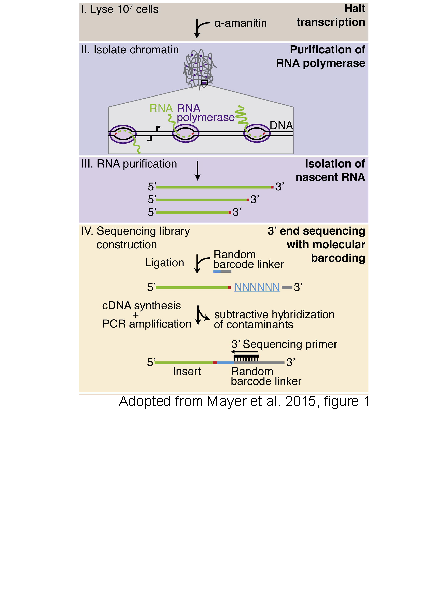
\includegraphics[trim=0 .5in 0
  0,clip,width=5in]{img/ch04/Figure1.pdf}
\caption[Graphical representation of NET-seq protocol]{\textbf{ Graphical representation of NET-seq protocol published in Mayer et al. \citep{mayer_native_2015}}  {\bf Panel I:} Halt transcription in cells with $\alpha$-Amantin. {\bf Panel II:} Purify chromatin containing PolII. {\bf Panel III:}  Purify nascent mRNA from chromatin fractionation. {\bf Panel IV:}  Library construction by adding DNA linker to 3' OH group, cDNA synthesis, and removal of mature mRNA contaminates}
\label{fig:ch04-protocol}
\end{figure}


\begin{figure}
\centering 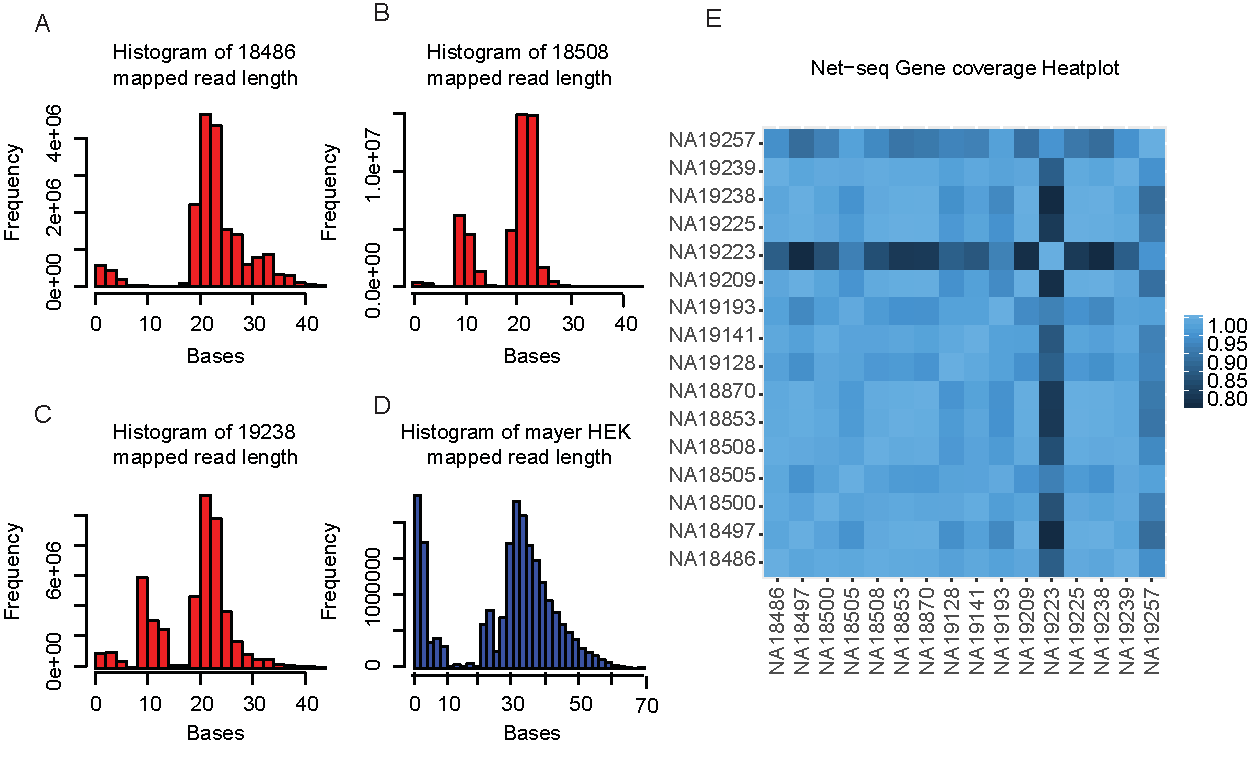
\includegraphics[trim=0 .3in 0
  0,clip,width=5in]{img/ch04/Figure2.pdf}
\caption[Quality control metrics for NET-seq libraries.]{\textbf{Quality control metrics for NET-seq libraries.} {\bf A} Histogram of mapped read lengths for NET-seq library NA18486. {\bf B} Histogram of mapped read lengths for NET-seq library NA18508. {\bf C} Histogram of mapped read lengths for NET-seq library NA19238. {\bf D} Histogram of mapped read lengths for NET-seq library generated from HEK cells and published in Mayer et al \citep{mayer_native_2015}). {\bf E} Pearson correlations for NET-seq library coverage in gene bodies. Coverage calculated as number of reads mapping to gene standardized by gene length.}
\label{fig:qualCont}
\end{figure}

We sequenced the libraries to an average depth of 160 million reads. For many libraries, less than 50\% of the reads mapped to the genome and once deduplicated based on UMIs, less than 5\% of sequenced reads were usable. Over 50\% of reads did not map because they were too short. Mapped reads from our libraries were shorter reads than those previously published (\citep{mayer_native_2015}, Figure \ref{fig:qualCont}A-D)


We next evaluated the mapped data on a genome wide scale. We assessed our data using the following metrics introduced by Meyer et al (mayer 2015). At the gene coverage level, NET-seq libraries were highly correlated (Figure \ref{fig:qualCont}E). Overall, we observed a bias toward read coverage at the 5' end of gene bodies (methods, Figure \ref{fig:genecov}A).  Within genes, we observed enrichment at 5' and 3' exon boundaries for the top 5\% of expressed exons (Figure \ref{fig:genecov}B, methods). After standardizing the number of reads mapping to each gene by gene length only, on average 42.7\% of genes were detected at greater than 0.001 standardized reads (Figure \ref{fig:genecov}C). Given the average gene length, 0.001 standardize reads represented about 65 reads. 


\begin{figure}
\centering 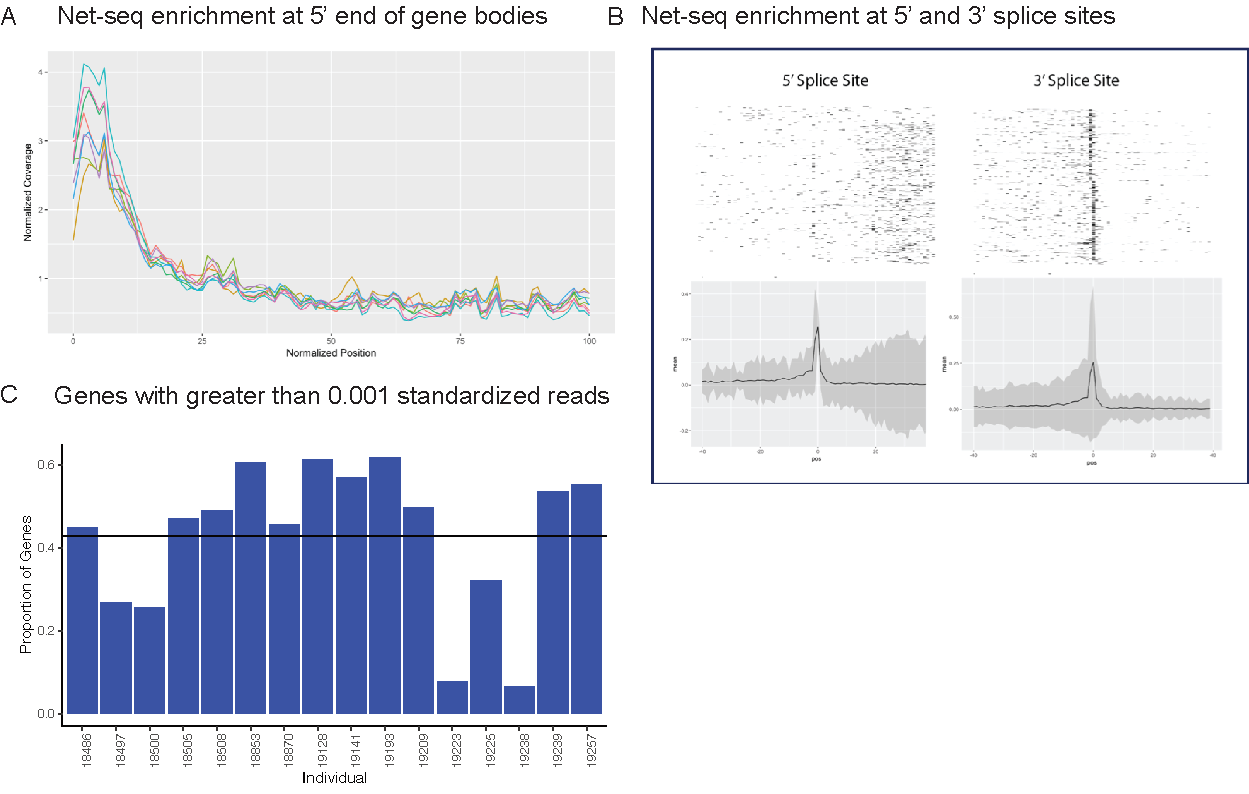
\includegraphics[trim=0 .3in 0
  0,clip,width=5in]{img/ch04/Figure3.pdf}
\caption[NET-seq Gene coverage.]{\textbf{NET-seq Gene coverage.} {\bf A} Enrichment for Distribution of read coverage along gene bodies calculated with Picard tools (NA18505, NA18508, NA18486, NA19239, NA19239, NA19141, NA19193, NA19257, NA19128). {\bf B}Histogram and smoothed density plots for NET-seq read coverage at 5' and 3' splice sites. {\bf C} Proportion of genes in each NET-seq library with greater than 0.001 standardized reads (methods).}
\label{fig:genecov}
\end{figure}


Our goal was to identify genomic regions with evidence for high PolII density and map genetic variation associated with variation in PolII elongation rate. In turn, we next explored coverage at individual gene loci. We used a wavelet-based Empirical Bayes shrinkage method implemented in smashr to denoise genic signal (\citep{xing_flexible_2016}, methods). For ACTB, the smoothing allowed us to identify regions of likely Pol II pausing at the TSS and splice sites (Figure \ref{fig:smash}). 



\begin{figure}
\centering 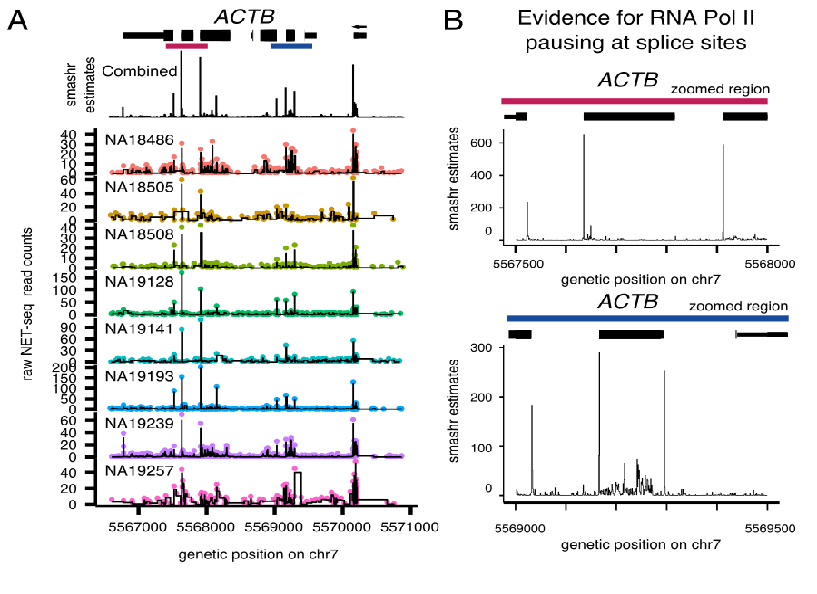
\includegraphics[trim=0 .3in 0
  0,clip,width=5in]{img/ch04/Figure4.pdf}
\caption[Smoothing of NET-seq data using smashr ]{\textbf{Smoothing of NET-seq data using smashr \citep{xing_flexible_2016}.} {\bf A} Raw counts along ACTB gene locus for 8 combined libraries (NA18505, NA18508, NA18486, NA19239, NA19239, NA19141, NA19193, NA19257, NA19128) as well as each library separately. {\bf B} Smoothed coverage along ACTB on combined NET-seq data. Signal at 5' and 3' splice sites.}
\label{fig:smash}
\end{figure}
 
Smoothing to differentiate signal from random noise would not account for contamination by mature mRNAs or technical mapping errors. We found evidence of many genomic locations, such as in the INSIG2 gene, with heavy read buildup. We were unable to identify technical or biological reasons for the high density of NET-seq reads (Figure \ref{fig:insig}). We hypothesize that unannotated chromatin associated mRNAs or low complexity repetitive reads. The protocol includes depletion of chromatin associated mature mRNAs, however the oligo pool is likely incomplete. Unannotated snoRNAs or snRNAs likely contribute to high density regions. Alternatively, because mapped reads are relatively short, repetitive genomic regions may be mipmapping, therefore contributing to regions of high read density. 

\begin{figure}
\centering 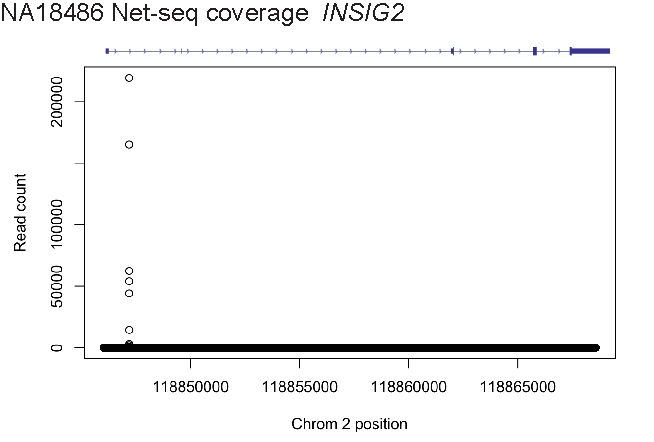
\includegraphics[trim=0 .3in 0
  0,clip,width=5in]{img/ch04/Figure5.pdf}
\caption[NA18486 NET-seq coverage along INSIG2 locus]{\textbf{NA18486 NET-seq coverage along INSIG2 locus}}
\label{fig:insig}
\end{figure}

We did not continue the analysis beyond these quality control metrics and low-level analyses. Further optimization of this protocol or another protocol is likely necessary to quantify Pol II pause pattern variation genome wide. 



\section{Discussion}\label{ch04-discussion}


By extracting and sequencing nascent chromatin-associated mRNA, we attempted to measure polymerase II (PolII) density and estimate transcription elongation rates a population of human LCLs. Using data from 16 individuals we were able to capture the broad patterns previously described by Mayer et al and others \cite{mayer_native_2015}. We found evidence for Poll II pausing at the TSS and at the 5' and 3' splice sites for highly expressed exons. We showed that in genes with high coverage, an Empirical Bayes shrinkage method could differentiate between regions of high PolII density and background random noise. Unfortunately, for most genes, we did not have high enough coverage to smooth the data. Further, we identified regions of the genome where a large proportion of the reads mapped for unknown technical reasons or biological contamination of mature chromatin associated mRNAs.

We believe the NET-seq libraries were of low quality and complexity for a number of reasons. The NET-seq protocol was difficult to optimize due to low concentration of input mRNA. Specifically, we needed to extract chromatin associated mRNA from 8 collections of 15 million cells to achieve the required 1$\mu g$ of input RNA. Moreover, the protocol included multiple gel extraction steps where lot of the mRNA was lost. While we explored alternative options, such as size selection with columns, none were specific enough for the desired fragments. Even after optimizing the protocol to achieve libraries of high enough concentration for sequencing, the nascent RNA fragments were shorter than reads published in Mayer et al \cite{mayer_native_2015}. We believe that while we selected the optimal fragment lengths, shorter fragments were preferentially incorporated and amplified into libraries. 

It is difficult to determine if our libraries were of lower quality than those published in Mayer et al because the published libraries also had a large number of un-mapped reads and a low signal-to-noise ratio. The authors largely characterized patterns across multiple genes did not collect a population sample to identify variation. It is likely that sequencing coverage played a large role in the differences between our results and those reported in Mayer et al \cite{mayer_native_2015}. For one replicated of HEK293T, they sequenced 1.2 billion reads with 555 million uniquely mapping. At this coverage, only 50\% of the reads had coverage of over 1 read per kilobase per million (RPKM) \cite{mayer_native_2015}. While we acknowledged that sequencing to this depth would be unreasonable in a population sample, we planned to take advantage of shared genotypes to identify genetic variants associated with PolII patterns. Unfortunately, our low coverage libraries were too noisy to confidently quantify PolII density, even if we merged on genotypes. 

We still believe that mapping genetic variants associated with PolII density would likely help in our understanding on gene regulation. There are a variety of alternative methods to collect nascent mRNA or PolII associated transcripts. Other potential methods largely fall into two classes. The first category relies on immunoprecipitation of PolII or a specific post translationally modified version of PolII \citep{nojima_mammalian_2015, gariglio_clustering_1981, buck_chip-chip_2004, kim_high-resolution_2005,wissink_nascent_2019, mayer_pause_2017}. These methods potentially suffer from non-specific binding of anti-bodies, and with the exception of mNetseq, are restricted to 200bp resolution \citep{nojima_mammalian_2015}. The second class of approaches utilize in-vitro incorporation of labeled nucleotides to identify regions of transcription potential. Transcription run-on assays, such as GRO-seq and PRO-seq, are vulnerable to variation in experimental conditions because the protocols include stopping and restarting transcriptions in non-physiological conditions \citep{kwak_precise_2013,core_analysis_2014, tome_single-molecule_2018, gardini_global_2017,mahat_base-pair-resolution_2016, mayer_pause_2017, wissink_nascent_2019}. 


To date, only one preprint has reported the usage of a variant of one of these methods to characterize nascent RNA in a population of human cell lines. $Kristj\grave{a}nsd\grave{o}ttir$ et al, quantified 5' capped nascent transcripts in 67 YRI LCLs with PRO-cap \citep{kristjansdottir_population-scale_2018}. In contrast to our work, these authors aimed to characterize transcription at enhancers and to identify genetic variation associated with enhancer transcription initiation. The authors also collected PRO-seq for 10 unique individuals \citep{kristjansdottir_population-scale_2018}. It is possible that once published, we or others could use these data to test for genetic variation associated with co-transcriptional PolII density variation. 


\section{Methods}\label{ch04-methods}



\subsection{Cell culture of LCLs}\label{cell-culture-of-LCLs} 

We cultured 16 human Epstein-Bar virus transformed lymphoblastoid cell lines (LCLs) in glutamine depleted RPMI (RPMI 1640 1X from Corning (15-040-CM)), completed with 15\% FBS, 2mM GlutaMax (Gibco (35050-061)), 100 $IU/ml$ Penicillin, and 100 $\mu g/mL$ Streptomyocin. We cultured all cells at 37C at 5\% CO2. The 16 cell lines represent a subset of the YRI individual LCLs collected as part of the hapmap project and are available through Coriell \citep{HapMap2005}. 
We used lines NA19527, NA19239, NA19238, NA19225, NA19223, NA19209, NA19193, NA19128, NA19141, NA19128, NA18853, NA18508, NA18505, NA18501, NA18497, NA18486. These lines also represent a subset of those used for the 3' sequencing published in Chapter 2 and in Mittleman et al. \citep{mittleman_alternative_2020}. 


\subsection{Collections and library preparation}\label{Collections-and-library-preparation}

After growing the LCLs to around 1 million cells per ml, we separated $1.5x10^{7}$ cells into 10 tubes, one for total cells, one for nuclear fraction and eight for the chromatin fraction. Collection dates and details can be found in Mittleman et al. Additional File 2 \cite{mittleman_alternative_2020}. We used the Native Elongating Transcript sequencing (NET-seq) collection protocol published in Mayer and Churchman 2016 with minor adjustments to three buffers \citep{mayr_evolution_2016}. Specifically, we added 1M $MgCl_{2}$ and 100\% Glycerol to the Cytoplasmic lysis buffer, Sucrose buffer, and the Nuclei wash buffer. We added the $MgCl_{2}$ to stabilize the nucleus and the glycerol as a freezing protectant. We halted transcription with $\alpha$-amanatin and separated the nuclear fraction using mild detergent and a sucrose cushion. We then separate the nucleoplasm from the chromatin using urea, salt, and a mild detergent. We then collected the chromatin through centrifugation and degradation of the DNA with a DNase treatment. We used the Qiagen miRNAeasy kit with manufacture instructions to extract mRNA from all three fractions.


We generated NET-seq library according to the Mayer and Churchman protocol with custom oligos ordered from IDT \citep{mayr_evolution_2016}. I captured the 3' end of chromatin associated mRNA molecules with a barcoded linker and convert the fragments into cDNA for library preparation. We sequenced each NET-seq library at the University Genomics Core facility using single end 50bp sequencing on the Illumina HiSeq4000 machine. We multiplexed 8 libraries together and sequenced each group on a total of 3 lanes. Custom sequencing primers can be found in Mayer and Churchman protocol \citep{mayr_evolution_2016}. 


\subsection{Data processing}\label{Data-processing}



We mapped all NET-seq libraries to GRCH37.75 downloaded from Ensemble using subjunc with default settings \citep{international_human_genome_sequencing_consortium_initial_2001, Liao2013} We used umi\_tools extract to extract the 6 base UMIs and umi-tools dedup to collapse duplicate reads \citep{smith_umi-tools_2017}. 
 
 We assessed computed genome coverage at basepair resolution using bedtools genomecov with the -d and -5 flags. We measured the coverage density along the gencode.v19 gene annotation using picard CollectRnaSeqMetrics \citep{frankish_gencode_2019,quinlan_bedtools_2010}. We used featureCounts with the -T 5 flag to quantify reads within the gencode.v19 gene annotation \citep{frankish_gencode_2019, Liao2014}. We used pysam to extract mapped read statistics from bam files \citep{Li2009}. We downloaded the HEK NET-seq published in Mayer et al. available from GEO under accession number GSE61332 \cite{mayer_genome-wide_2016}.  We re-processed the fastq file using our mapping pipeline. We used the smash.pois function with the EM algorithm in the smashr package on individual genes for signal denoising \citep{xing_flexible_2016}. The function implemented a wavelet-based Empirical Bayes shrinkage method \citep{xing_flexible_2016}. 

We attempted to recreate a version of Mayer et al. figure 7 using NA18486 sequence coverage for this analysis \cite{mayer_genome-wide_2016}. Due to low library coverage and complexity, we did not separate the exons into, constitutive, alternatively retained, alternative skipped. We quantified coverage at base pair resolution for 40bp upstream and downstream of the 5' and 3' splice sites of the top 5\% covered exons. We then standardized base pair coverage by exon coverage.   
